
\documentclass{article}
\author{fblazco}
\title{IIC2343}
\usepackage{amsmath}
\usepackage{graphicx}
\begin{document}
	\maketitle
    \section{Clase 1}
    \begin{enumerate}
        \item \textbf{Fecha Evaluaciones}
    \end{enumerate}    
    \section{Clase 2}
    \section{Clase 3}
    \begin{enumerate}
        \subsection{Compuertas}
        \item La compuerta NOT es un relee con salida not(A), y entradas A y corriente
        \item Lacompuerta OR se compone de 2 relee juntos (hacer tablita)
        \item La compuerta AND son dos relee consecutivos (en secuencia) donde el segundo esta conectado a la corriente del primero
        \item Propuesto: Definir \begin{enumerate}
            \item XOR, 
            \item   NAND 
            \item NOR 
            \item XNOR
        \end{enumerate}  usando reeles
    \end{enumerate}
        \subsection{HALF-ADDER}
        \begin{enumerate}
            \item Recibe dos señales de entrada y entrega 2 señales de salida, el Carry y el S (permite sumas de 1 bit sin tomar en cuenta el Carry)
           \item \begin{figure}
                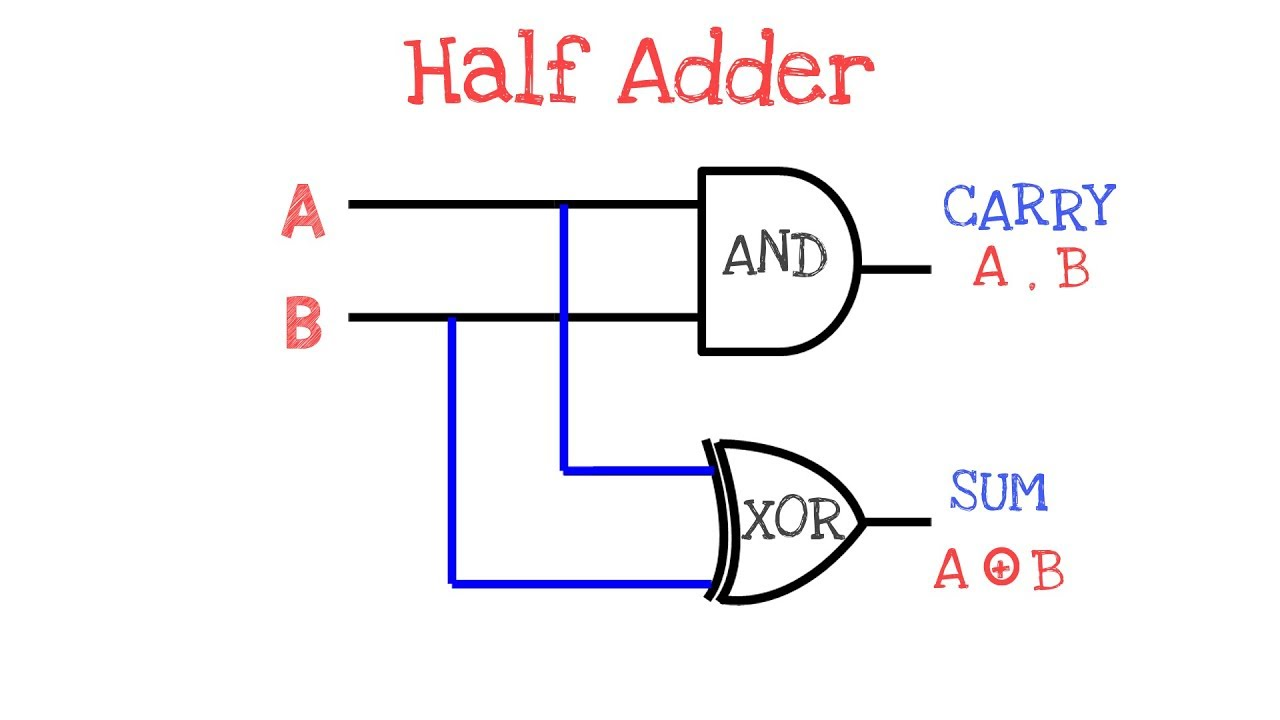
\includegraphics[width=300px]{halfadder.jpg}
                \caption{HF}
                \label{fig:HALF-ADDER}
            \end{figure}
        \end{enumerate}
        
        \subsection{FULL-ADDER}
            \begin{enumerate}
                \item Un full adder esta compuesto de 2 HALF-ADDER, esto nos permite realizar la suma entre 2 bits, considerando el Carry
            \end{enumerate}
             \begin{figure}
                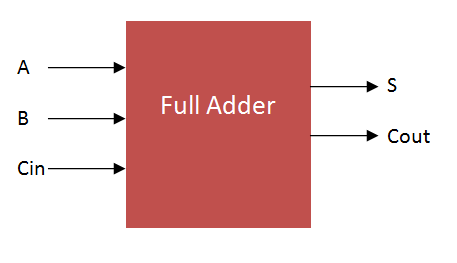
\includegraphics[width=250px]{fulladder.png}
                \caption{HF}
                \label{fig:Full-adder}
            \end{figure}
        \subsection{Sumador de 4bits}
        \begin{figure}
            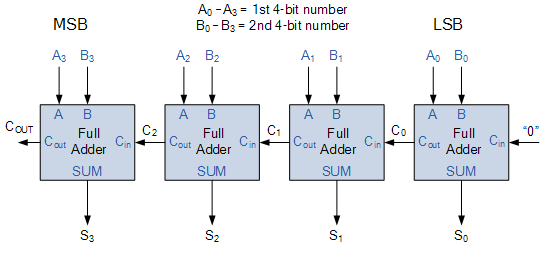
\includegraphics[width=300px]{sumador4bits.png}
            \caption{HF}
            \label{fig:Sumador 4bits}
        \end{figure}
        \begin{enumerate}
            \item Concatenando n full-adders, podemos crear sumadores de n bits, respetando el acarreo
            \item 
        \end{enumerate}
        \section{Clase 4}
        \subsection{Minterms y Maxterms}
        \textbf{Minterm}
        \begin{enumerate}
            \item Las señales dentro de una combinacion de input se conectan con compuertas AND
            por que se debe verificar que sus valores son los esperados.
            A las señales de valor 0 se les aplica NOT para verificar que tengan un valor de verdad falso
            \item Todas las combinaciones se conectan con OR's 
            \item \begin{equation}
                ( \bar{A} \wedge B \wedge \bar{C}) \vee 
                ( A \wedge \bar{B} \wedge C) \vee  
                ( A \wedge B \wedge C)
            \end{equation}  
        \end{enumerate}
        \textbf{Maxterm}
        \begin{enumerate}
            \item funcion similar a un Minterm (rellenar)
            \item \begin{equation}
                \begin{aligned}
                    ( \bar{A} \wedge B \wedge \bar{C}) \\
                    ( \bar{A} \wedge B \wedge \bar{C}) \\
                    ( \bar{A} \wedge B \wedge \bar{C}) \\ 
                    ( \bar{A} \wedge B \wedge \bar{C}) \\
                    ( \bar{A} \wedge B \wedge \bar{C}) 
                \end{aligned}
            \end{equation}
        \end{enumerate}
        \newpage
        \subsection{Unidad aritmetico logica ALU}
        \textbf{Circuitos de Control}
        \begin{enumerate}
            \item Enabler o habilitador: \begin{center}
                 -Componente que habilita o no el paso de una señal o bus de datos
            
            \end{center}
            \item Multiplexor o MUX:  \begin{center}
                -Permite el paso de una señal o bus de datos entre un conjunto de opciones. 
                Se construye como una extension del \textbf{enabler}
            \end{center}
            \item De-Multiplexor o Demux: \begin{center}
                -Transmite una señal o bus de datos a una de multiples salidas
            \end{center}
        \end{enumerate}
\end{document}  



